\documentclass[conference]{IEEEtran}
\IEEEoverridecommandlockouts
% The preceding line is only needed to identify funding in the first footnote. If that is unneeded, please comment it out.
\usepackage{cite}
\usepackage{amsmath,amssymb,amsfonts}
\usepackage{algorithmic}
\usepackage{graphicx}
\usepackage{textcomp}
\usepackage{xcolor}
\usepackage{tabularx}
\usepackage{multirow}
\usepackage{graphics} % for pdf, bitmapped graphics files
\usepackage{subfig}
\usepackage{subcaption}
\usepackage{hyperref}
\usepackage{academicons}
\usepackage{xcolor}
\usepackage{listings}
\usepackage{tabularx} % Asegúrate de incluir este paquete

\usepackage{tikz}
\usetikzlibrary{shapes.geometric, arrows}

\usetikzlibrary{shapes.geometric, arrows}

\tikzstyle{startstop} = [rectangle, rounded corners, minimum width=3cm, minimum height=1cm,text centered, draw=black, fill=red!30]
\tikzstyle{process} = [rectangle, minimum width=3cm, minimum height=1cm, text centered, draw=black, fill=blue!30]
\tikzstyle{arrow} = [thick,->,>=stealth]


\def\BibTeX{{\rm B\kern-.05em{\sc i\kern-.025em b}\kern-.08em
		T\kern-.1667em\lower.7ex\hbox{E}\kern-.125emX}}

% Color Enlace
\definecolor{colorEnlace}{RGB}{0, 0, 0}
\hypersetup{
	colorlinks=true,
	linkcolor=colorEnlace,
	citecolor=colorEnlace,
	urlcolor=colorEnlace,
	pdfauthor={Davis Bremdow Salazar Roa},
	pdftitle={Sistemas Embebidos}
}
\definecolor{mybg}{rgb}{0.97,0.97,0.97}
\definecolor{mygray}{gray}{0.4}
\definecolor{mygreen}{rgb}{0,0.6,0}
\definecolor{myblue}{rgb}{0,0,0.8}
\definecolor{mypurple}{rgb}{0.58,0,0.82}
\definecolor{myred}{rgb}{0.7,0,0}

\lstdefinelanguage{MatlabEnhanced}{
	language=Matlab,
	morekeywords={[2]linspace,plot,title,xlabel,ylabel,legend,grid},
	morekeywords={[3]sin,cos,exp,log,sqrt},
	keywordstyle=\color{myblue}\bfseries,
	keywordstyle=[2]\color{mypurple},
	keywordstyle=[3]\color{myred},
	commentstyle=\color{mygreen}\itshape,
	stringstyle=\color{mygray},
	morecomment=[l]%
}

\lstset{
	language=MatlabEnhanced,
	backgroundcolor=\color{mybg},
	frame=single,
	basicstyle=\ttfamily\small,
	showstringspaces=false,
	numbers=none,              %
	xleftmargin=0pt,           %
	framexleftmargin=0pt,      
	framexrightmargin=0pt,
	framextopmargin=2pt,
	framexbottommargin=2pt,
	breaklines=true,
	tabsize=1,
}

% Control 
\usepackage{amsmath}
\begin{document}
	
	\title{Modulación FM - Análisis de parámetros}
	\author{
		\makebox[\textwidth][c]{\large\textbf{Universidad Nacional de San Antonio Abad del Cusco}}\\
		\makebox[\textwidth][c]{\normalsize\textit{Escuela profesional de Ingeniería Electrónica}}\\
		\makebox[\textwidth][c]{\normalsize\textit{Laboratorio de Circuitos Electrónicos III}}\\
		\and
		\IEEEauthorblockN{Ing. Milton Velasquez Curo}
		\IEEEauthorblockA{Ingeniero Electrónico \\
			Cusco, Perú \\
			milton.velasquez@unsaac.edu.pe}
		\and
		\IEEEauthorblockN{Ruth Juana Espino Puma - 185746}
		\IEEEauthorblockA{Estudiante de Ingeniería Electrónica \\
			Cusco, Perú \\
			184657@unsaac.edu.pe}
		\and
		\IEEEauthorblockN{Davis Bremdow Salazar Roa - 200353}
		\IEEEauthorblockA{Estudiante de Ingeniería Electrónica \\
			Cusco, Perú \\
			200353@unsaac.edu.pe}
	}
	
	\maketitle
	\begin{abstract}
		La modulación es un proceso fundamental en las telecomunicaciones que consiste en variar una o más propiedades de una señal portadora (como amplitud, frecuencia o fase) en función de una señal de información o mensaje. Este proceso permite transmitir información a largas distancias de manera eficiente, minimizando interferencias y aprovechando mejor el espectro de frecuencias. Existen varios tipos de modulación, entre ellos la modulación en amplitud (AM), frecuencia (FM) y fase (PM), cada una con características y usos específicos según las necesidades del sistema de comunicación.
		
	\end{abstract}
	
	\begin{IEEEkeywords}
		Modulación, portadora, señal, índice de modulación, amplitud, frecuencia, fase, transmisión, espectro, distorsión.
	\end{IEEEkeywords}
	
	%% Contenido del documento
	
	\section{Modulación en frecuencia.}
	La modulación en frecuencia (FM) es una técnica aplicada en los sistemas de comunicación por radio. Consiste en variar la frecuencia de una señal portadora en función de la información que se desea transmitir, con amplitud constante. Es asi que  los datos o señales, como el audio, se integran a la portadora mediante cambios proporcionales en su frecuencia, permitiendo una transmisión más eficiente frente al ruido y las interferencias.
	\begin{figure}[h]
		\centering
		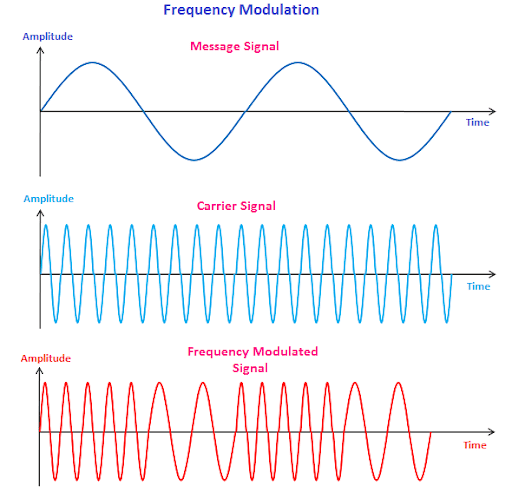
\includegraphics[width=0.5\textwidth]{media/modulacion-fm}
		\caption{Modulacion en frecuencia.}
		\label{fig:enter-label}
	\end{figure}
	\section{Ecuacion general de la modulacion en frecuencia}
	La siguiente funcion, representa la señal basica FM.
	\[
	s(t) = A_c \cos\left(2\pi f_c t + \beta \sin(2\pi f_m t)\right)
	\]
	\begin{itemize}
		\item $s(t)$: Señal modulada en frecuencia.
		\item $A_c$: Amplitud de la onda portadora, constante.
		\item $f_c$: Frecuencia de la portadora (en Hz), alrededor de la cual se producen las desviaciones.
		\item $f_m$: Frecuencia de la señal moduladora (Hz).
		\item $\beta$: Índice de modulación.
		\item $\Delta f$: Desviación máxima de frecuencia.
		\item $\sin(2\pi f_m t)$: Señal moduladora senoidal.
	\end{itemize}
	\section{Parametros de Modulacion en frecuencia.}
	\subsection{Indice de Modulacion}
	Es la relación de la desviación de frecuencia máxima a la frecuencia de señal de modulación más alta.
	\begin{equation}
		m = \frac{\Delta f}{f_m}
		\label{eq:indice-modulacion}
	\end{equation}
	
	\subsection{Maxima desviacion en frecuencia.}
	Es el mayor cambio que puede sufrir la señal portadora  debido a la modulación.
	\begin{equation}
		\Delta f= \frac{K V_m}{2\pi}
		\label{eq:max-desviacion-frecuencia}
	\end{equation}
	
	\subsection{Ancho de banda}
	Es un factor central que afecta tanto la calidad como la eficiencia de los sistemas de comunicación.Está determinado principalmente por la desviación de la frecuencia y la frecuencia de la señal de modulación, creando bandas laterales a cada lado del portador.
	\[
	BW = {2}{f_m}{N}
	\label{eq:ancho-banda}
	\]
	\subsubsection{Regla de Carson para el ancho de banda.}
	La regla de Carson estima el ancho de banda necesario para una señal modulada en frecuencia. Toma en cuenta tanto la desviación de frecuencia como la frecuencia máxima del mensaje, y es válida especialmente cuando el índice de modulación $\beta > 1$.
	\[
	BW = 2(\Delta f + f_m)
	\]
	\begin{itemize}
		\item $BW$: Ancho de banda total de la señal FM ( Hz).
		\item $\Delta f$: Desviación máxima de frecuencia ( Hz).
		\item $f_m$: Frecuencia máxima de la señal moduladora (Hz).
	\end{itemize}
	
	\subsection{Porcentaje de modulacion}
	Se refiere a la razon de la desviacion  de frecuencia  efectiva con la  desviacion de la frecuencia  maxima permisible.
	\[
	\text{Porcentaje de modulación} = \left( \frac{\Delta f}{\Delta f_{\text{máx}}} \right) \times 100\%
	\]
	
	\section{Ventajas y Desventajas de la Modulacion FM}
	Ventajas.
	\begin{itemize}
		\item Alta inmunidad al ruido, menos suceptibilidad a interferencias.
		\item Mantiene una buena calidad de la señal.
		\item Asegura la comunicacion aun en movimiento. 
	\end{itemize}
	Desventajas.
	\begin{itemize}
		\item Mayor  uso de ancho e banda,  requiere mas espectro  que otras tecnicas de modulacion.
		\item Complejos y costosos, equipos que detectan con mayor precision.
		\item Requieren un filtrado preciso,para evitar interferencias y perdida de calidad.
	\end{itemize}
	
	\section{Modulación FM}
	
	Como se pudo apreciar anteriormente la modulación FM contempla una relación entre la frecuencia con la integral de la moduladora, esto se puede apreciar en las ecuaciones anteriormente definidas.
	
	Por lo tanto para poder expresar a nivel digital este procedimiento, se debe tener en cuenta 2 parámetros fundamentales, siendo estos, los siguientes:
	
	\begin{itemize}
		\item Integral de la señal de información
		\item Señal portadora
		\item Función de Bessel (Análisis en frecuencia)
	\end{itemize}
	
	Una primera aproximación al análisis FM, nos muestra los primero parámetros de interés como la desviación de frecuencia, el índice de modulación y dentro del propio análisis digital parámetros como la frecuencia o periodo de muestreo se deben considerar para un correcto análisis de datos y resultados.
	
	\subsection{Desviación de frecuencia}
	Como se define en \ref{eq:max-desviacion-frecuencia} este parámetro define el cambio en la frecuencia de la señal portadora en función a la moduladora, generando los cambios de frecuencia en la señal alterando la periodicidad de la señal resultante cuando la señal moduladora alterna su valor de voltaje.
	
	\begin{figure}[h]
		\centering
		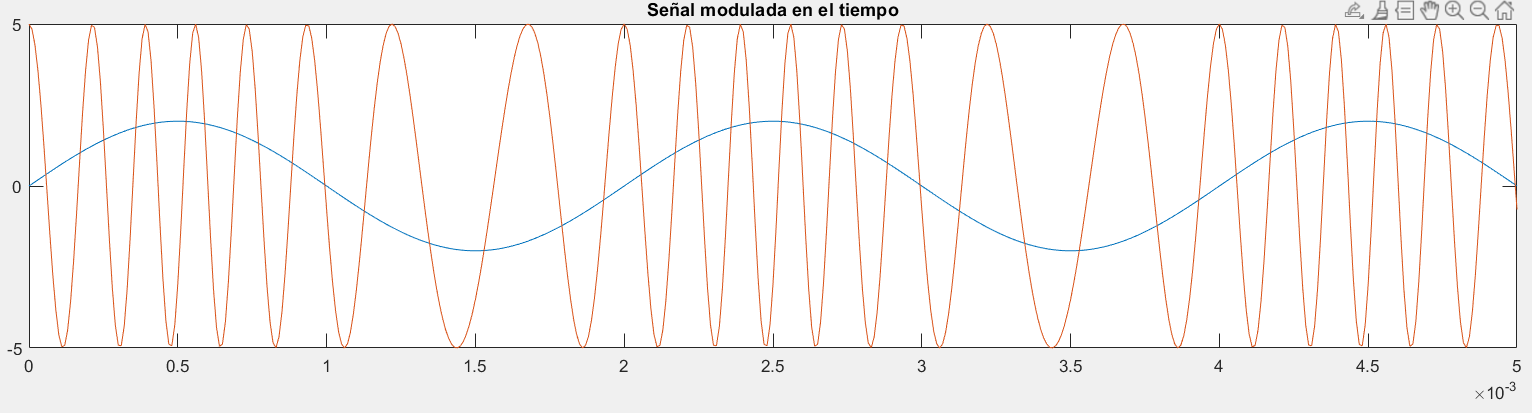
\includegraphics[width=0.5\textwidth]{media/forma-alterada-fm}
		\caption{Modulación FM}
		\label{fig:forma-alterada-fm}
	\end{figure}
	
	Esto se puede apreciar en la figura \ref{fig:forma-alterada-fm} que muestra este comportamiento para el cambio de polaridad o excursión negativa de la señal de información.
	
	\subsection{Índice de modulación}
	
	Por otro lado una modificación del índice de modulación definido en \ref{eq:indice-modulacion} de igual forma que la desviación de frecuencia implicará un cambio en la forma de onda resultante en la modulación, sin embargo se debe tener en cuenta que para este parámetro también se toma en consideración la frecuencia de la señal información.
	
	Por ejemplo para una frecuencia $f_m = 700 [Hz]$ y una amplitud $a = 5$, la señal FM resultante tiene un cambio más pronunciado durante la excursión negativa como se muestra en la figura \ref{fig:mod-indice-modulacion} esto debido a que se tiene una mayor desplazamiento de frecuencia en relación a la amplitud del voltaje.
	
	\begin{figure}[h]
		\centering
		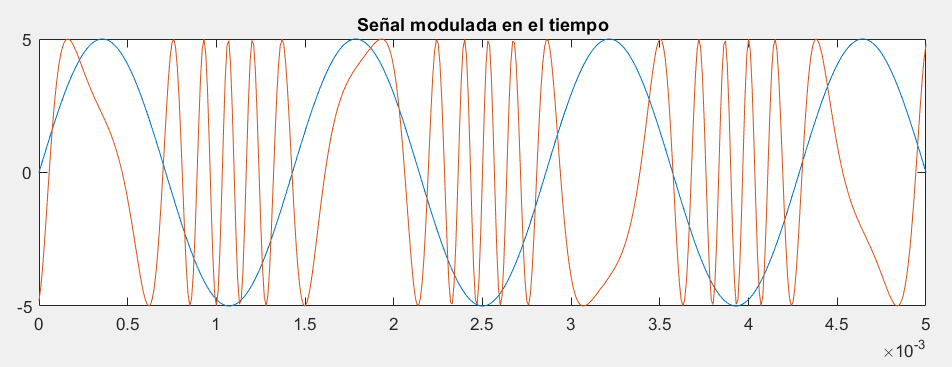
\includegraphics[width=0.5\textwidth]{media/mod-indice-modulacion}
		\caption{Señal FM resultante al modificación del índice de modulación}
		\label{fig:mod-indice-modulacion}
	\end{figure}
	
	\section{Análisis en frecuencia}
	
	Un análisis en el dominio de la frecuencia requiere además de la transformada rápida de Fourier, la consideración matematica en torno a la expresión de Bessel debido al proceso NO lineal requerido por la modulación FM.
	
	Para ello al desarrollar las expresiones complejas de este análisis se obtiene la expresión general mostrada en \ref{eq:bessel} citado en \cite{stremler2006}
	
	\begin{equation}
		\phi_{\textrm{FM}}(t) = A \sum_{n=-\infty}^{\infty} J_n(\beta) \, \cos\, (\omega_c + n\omega_m) t
		\label{eq:bessel}
	\end{equation}
	
	La cual generaliza una señal FM en función a $J_n(\beta)$ (función de Bessel) y una suma infinita de tonos múltiplos o armónicos de la frecuencia angular de la señal de información.
	
	Finalmente analizar la señal FM modulada en frecuencia, se aplicará la transformada de Fourier a la expresión \ref{eq:bessel} considerando para ello la función de Bessel como una constante que modificara la amplitud de la senoidal perteneciente a la portadora.
	
	\begin{figure}[h]
		\centering
		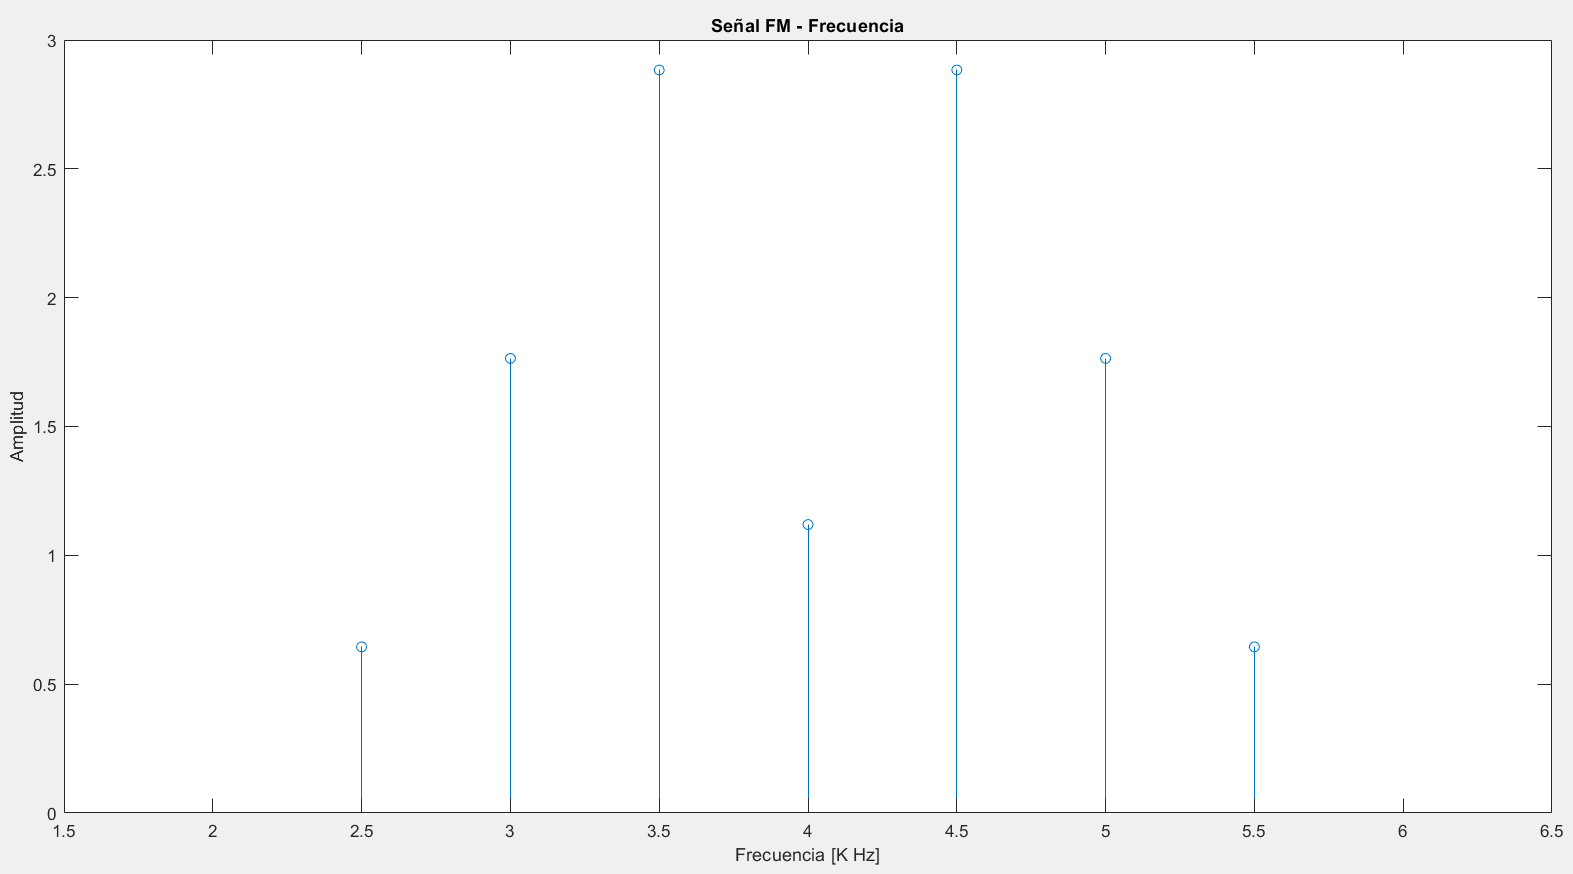
\includegraphics[width=0.5\textwidth]{media/fm-frecuencia-bessel}
		\caption{Señal FM - Frecuencia}
		\label{fig:fm-frecuencia-bessel}
	\end{figure}
	
	\section{Simulación en MATLAB}
	
	La generación de cada señal así los procesos matemáticos para la modulación se muestra en el listing \ref{lst:modulacion-fm}
	
	\begin{lstlisting}[caption="Modulación FM", numbers=none, label=lst:modulacion-fm]
		clc, clear, close all;
		
		%% Variables globales 
		Fs = 100000;
		t = 0: 1/Fs: 0.5*10^-2; % Determina la cantidad de puntos
		
		%% Senal de informacion;
		a = 2;
		fm = 500;
		ft = a*sin(2*pi*fm*t);
		
		%% Senal Fm modulada
		A = 5;
		fc = 4000;
		fdev = 1000;
		% fi = A*fmmod(ft, fc, Fs, fdev, 0);
		
		fi = A*sin(2*pi*fc*t + a*cos(2*pi*fm*t));
		
		%% Dominio del tiempo
		
		figure
		subplot(2,1,1);
		plot(t, ft);
		hold on
		plot(t, fi);
		title("Senal modulada en el tiempo");
		hold off
		
		%% Dominio de la Frecuencia
		N = length(t);
		FI = fftshift(fft(fi));
		
		% f = fs*(0:N-1)/N;
		f = linspace(-Fs/2, Fs/2, N);
		
		subplot(2, 1, 2);
		stem(f, abs(FI/N));
		title("Senal expresada en el dominio de la frecuencia");
		
		%% Analisis en frecuencia - Bessel
		
		fc = fc/1000;
		fm = fm/1000;
		
		Ffm(1) = 0;
		y(1) = 0;
		figure
		j = 1;
		
		for i = -3 : 3
		Ffm(j) = A*besselj(i,a);
		if( i < 0)
		y(j) = fc + i*fm;
		elseif(i == 0)
		y(j) = fc;
		else
		y(j) = fc + i*fm;
		end
		j = j + 1;
		end
		
		stem(y, abs(Ffm));
		title("Senal FM - Frecuencia");
		xlabel("Frecuencia [K Hz]");
		ylabel("Amplitud");
		xlim([1.5, 6.5]);
	\end{lstlisting}
	
	Definiéndose en la primera etapa los vectores de tiempo, frecuencia de muestreo, seguidamente se tiene la definición de las señales sinusoidales para finalmente realizar el gráfico de la modulación en función a las características para realizar este proceso, ubicándose finalmente el análisis en frecuencia de la señal.
	
	\bibliographystyle{IEEEtran}
	\bibliography{biblio}
\end{document}
